\documentclass[12pt, titlepage]{report}
\usepackage{consumer_resource_final}
\graphicspath{{./figures/}}

\begin{document}
\begin{figure}[h!]
\centering
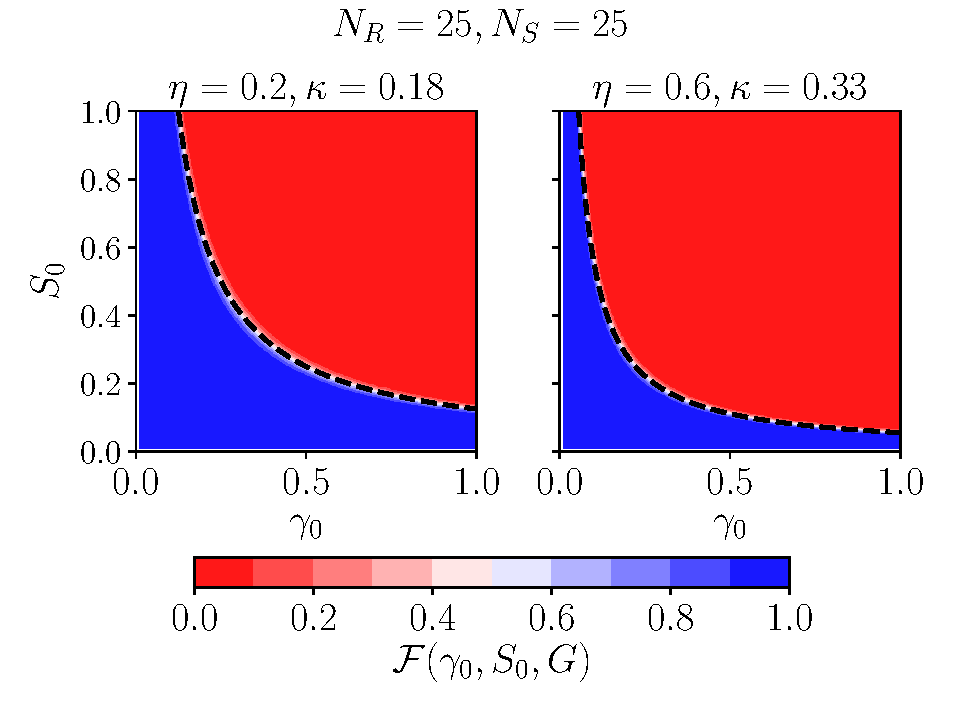
\includegraphics[width=0.7\linewidth]{typical_feasibility_volume}
\caption{Plot of the feasibility region in the absence of syntrophy. The color curve indicates the feasibility function $\mathcal{F}\left((\gamma_0, S_0, \alpha_0=0), G, 0\right)$ for $G_1$, which has a connectance $\kappa_{G}=0.18$ and ecological overlap $\eta_{G}=0.2$ (left) and $G_2$ with $\kappa_G=0.28$ and $\eta_G=0.4$(right). We observe a steep descent which marks a very clear transition from a totally feasible regime to a totally unfeasible regime, which allows us to precisely get the boundary of $\mathcal{F}^{G, 0}_1$. The dashed lines indicate the theoretical predictions.}
\label{fig: typical feasibility region}
\end{figure}
\begin{figure}[h!]
	\captionsetup[subfigure]{captionskip = -165pt, margin = 45pt}
\subfloat[\label{fig: deviation away from theory feasibility fixed nestedness}]{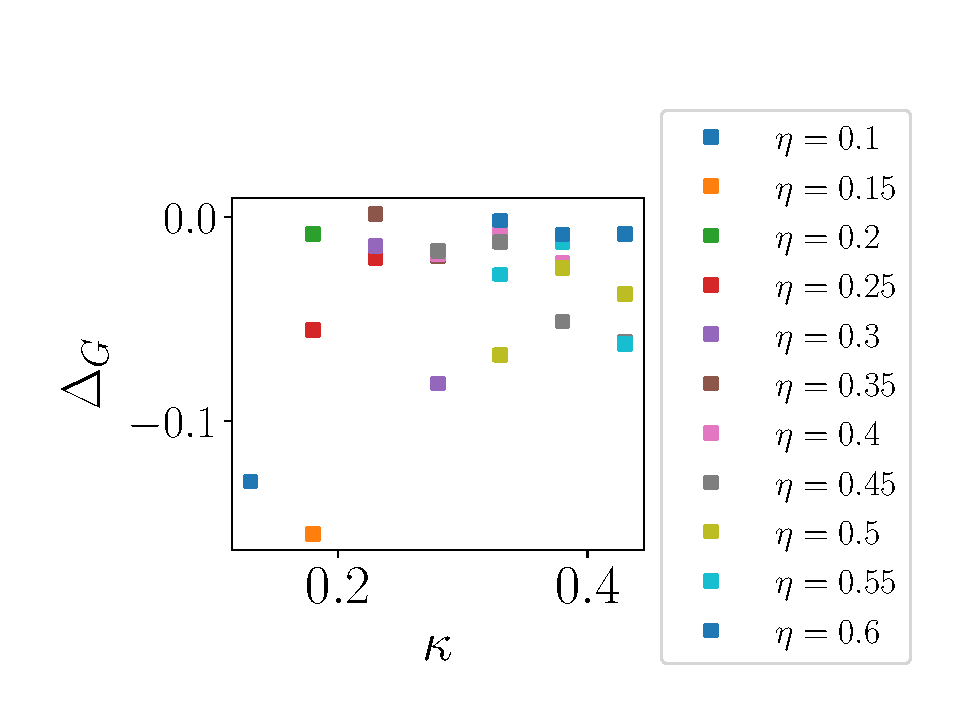
\includegraphics[width=0.49\linewidth]{feasibility_away_from_theory_fixed_nestedness}}
\captionsetup[subfigure]{captionskip = -175pt, margin = 45pt}
\subfloat[\label{fig: deviation away from theory feasibility fixed connectance}]{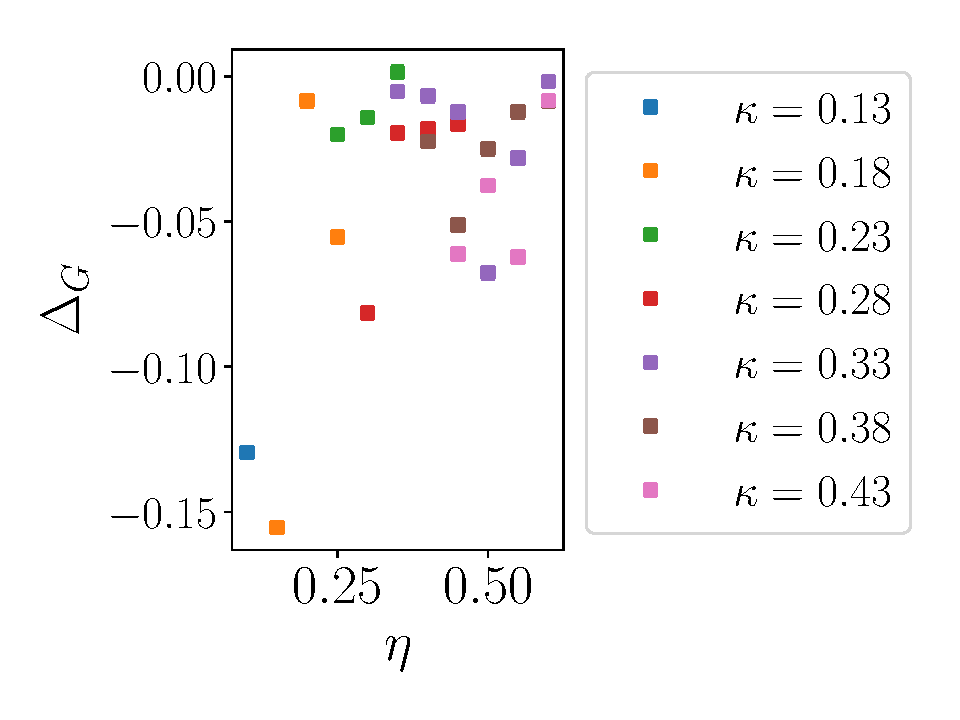
\includegraphics[width=0.49\linewidth]{feasibility_away_from_theory_fixed_connectance}}
\caption{Relative error in the determination of the boundary of $\mathcal{F}^{G,0}_1$ (a) varying connectance at fixed ecological overlap and (b) varying ecological overlap at fixed connectance. The theoretical prediction tends to overestimate the measured value. The larger the ecological overlap or connectance, the better the estimate.}\label{fig: deviation away from theory feasibility}
\end{figure}
\begin{figure}[h!]
\centering
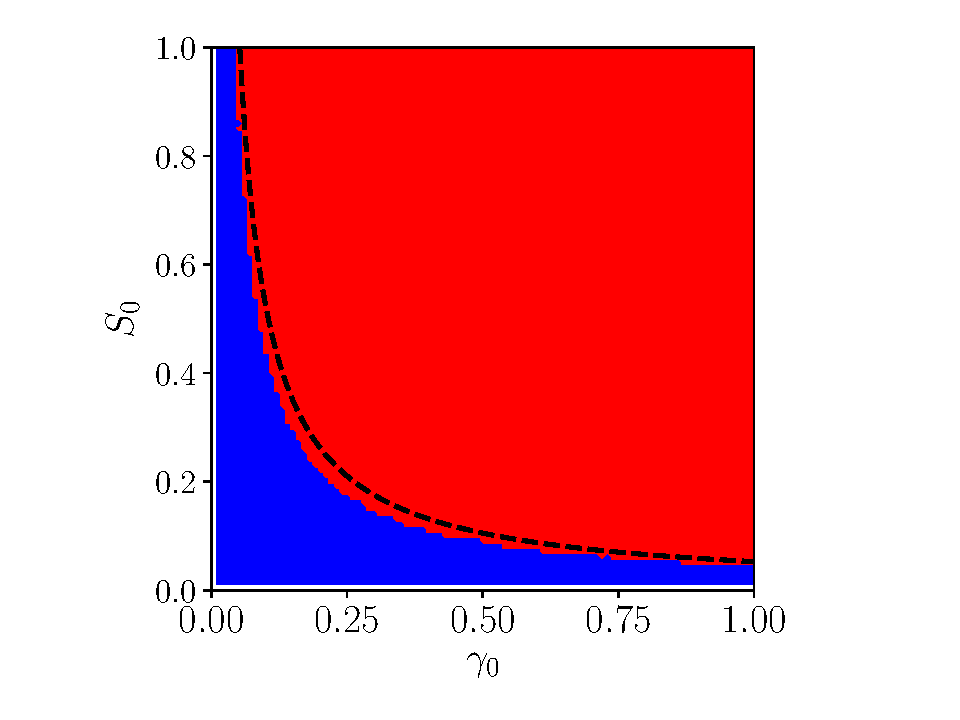
\includegraphics[width=0.6\linewidth]{common_feasibility_volume_no_syntrophy}
\caption{Plot of the common feasibility region. The blue area indicates the common feasibility volume, computed numerically, while the dashed line shows the analytical prediction. Although the match is not as good as before, the relative error is only of the order of $20 \%$. The red part is the area where not all matrices are fully feasible.}
\label{fig: common feasible volume no syntrophy}
\end{figure}
\begin{figure}
\captionsetup[subfigure]{captionskip = -195pt, margin=65pt}
\hspace{-0.2\linewidth}
\subfloat[\label{fig: feasibility results feasibility region eta 0.6 kappa 0.3 NR=25}]{\includegraphics[width=1.4\linewidth]{{feasibility_region_wt_wc_NR25_NS25_Nest0.6_Conn0.3168}.pdf}}

\vspace{-60pt}
\hspace{-0.2\linewidth}
\subfloat[]{\includegraphics[width=1.4\linewidth]{{feasibility_region_wt_wc_NR25_NS25_Nest0.35_Conn0.2208}.pdf}}

\vspace{-60pt}
\hspace{-0.2\linewidth}
\subfloat[]{\includegraphics[width=1.4\linewidth]{{feasibility_region_wt_NR25_NS25_Nest0.15_Conn0.1808}.pdf}}

\caption{Fully feasible region in the $(\gamma_0,S_0) \in [0,1] \times [0,1]$ unit square as a function of syntrophy for different consumption matrices $G$: (a)
$\eta_G=0.6$, $\kappa_G=0.32$, (b) $\eta_G=0.35$, $\kappa_G=0.22$ and (c) $\eta_G=0.15$, $\kappa_G=0.18$.
The white zone corresponds to points that are never fully feasible. The colour of a given point tells until which syntrophy that point is fully feasible, \eg
a light blue point is fully feasible for $0 \leq \alpha_0 \leq \num{9.1e-3}$. The size of the feasibility regions depend heavily on the topology of the matrix, which makes the problem far from trivial.}\label{fig: feasibility results fully feasible volume different consumption matrices}
\end{figure}
\begin{figure}
\centering
\includegraphics[width=0.6\linewidth]{{size_feasibility_region_NR25_NS25_Nest0.25_Conn0.2336}.pdf}
\caption{Decay of the volume of the fully feasible region $\mathcal{F}^{G,A}_1(\alpha_0)$ for a matrix consumption $G$ with ecological overlap $\eta_G=0.25$ and connectance $\kappa_G=0.23$ on a logarithmic scale. The solid lines represent the exponential fit explained in the main text. The four different colors represent the four different structures considered for the syntrophy matrix. The decay of $\text{Vol}(\mathcal{F}^{G,A}_1(\alpha_0))$ seems well approximated by an exponential decay. A random syntrophy matrix (RS scenario) allows for a larger feasibility volume.}
\label{fig: feasibility results typical shrinkage of feasible volume}
\end{figure}
\begin{figure}
\captionsetup[subfigure]{captionskip=-190pt, margin=44pt}
\hspace{-0.05\linewidth}
\subfloat[]{\includegraphics[width=0.55\linewidth]{{feasibility_NR25_NS25_feasibility_decay_rate_fixed_nestedness_fully_connected}.pdf}}
\subfloat[]{\includegraphics[width=0.55\linewidth]{{feasibility_NR25_NS25_feasibility_decay_rate_fixed_connectance_fully_connected}.pdf}}
\caption{Feasibility decay rate $d_F(G,A)$ for $A$ fully connected and $(G,A)\in S_{25}$. (a) $d_F$ as a function of the connectance of $G$ for different fixed ecological overlaps and (b) $d_F$ as a function of the ecological overlap $\eta_G$ for fixed different connectances. A strong trend may be seen: at fixed ecological overlap, $d_F$ decreases with connectance and at fixed connectance it increases with ecological overlap. Since a small $d_F$ allows to sustain a larger syntrophy, microbial communities where syntrophic interactions play a large role will tend to have a high connectance of the consumption matrix and a low ecological overlap.}\label{fig: feasibility results decay rate FC case}
\end{figure}
\begin{figure}
\captionsetup[subfigure]{captionskip=-180pt, margin=44pt}

\vspace{-30pt}
\hspace{-0.03\linewidth}
\subfloat[]{\includegraphics[width=0.53\linewidth]{{feasibility_NR25_NS25_feasibility_decay_rate_dev_away_from_FC_fixed_nestedness_no_release_when_eat}.pdf}}
\subfloat[]{\includegraphics[width=0.53\linewidth]{{feasibility_NR25_NS25_feasibility_decay_rate_dev_away_from_FC_fixed_connectance_no_release_when_eat}.pdf}}

\vspace{-12pt}
\hspace{-0.03\linewidth}
\subfloat[]{\includegraphics[width=0.53\linewidth]{{feasibility_NR25_NS25_feasibility_decay_rate_dev_away_from_FC_fixed_nestedness_optimal_matrix}.pdf}}
\subfloat[]{\includegraphics[width=0.53\linewidth]{{feasibility_NR25_NS25_feasibility_decay_rate_dev_away_from_FC_fixed_connectance_optimal_matrix}.pdf}}

\vspace{-12pt}
\hspace{-0.03\linewidth}
\subfloat[]{\includegraphics[width=0.53\linewidth]{{feasibility_NR25_NS25_feasibility_decay_rate_dev_away_from_FC_fixed_nestedness_random_structure}.pdf}}
\subfloat[]{\includegraphics[width=0.53\linewidth]{{feasibility_NR25_NS25_feasibility_decay_rate_dev_away_from_FC_fixed_connectance_random_structure}.pdf}}
\vspace{-6pt}
\caption{Relative difference of the feasibility decay rate for the considered $A$ scenario compared to the FC null case (Fig.\ref{fig: feasibility results decay rate FC case}) for $N_R=25$ and $N_S=25$. Plots on the first column (a)-(c)-(e) show how that quantity changes with connectance for a given ecological overlap, while plot on the second column (b)-(d)-(f) show how it evolves when ecological overlap is changed and connectance is kept fixed. Different structures of the $A$ matrix are considered: (a)-(b) NIS, (c)-(d) LRI (e)-(f) RS. A positive $y$-coordinate means that for the feasibility decay rate of the current syntrophy scenario is smaller than for the FC case, \ie the system sustains syntrophy better with the considered $A$-structure compared to fully connected. Apart from a few marginal exceptions, the FC scenario is always outperformed by the other scenarios, especially the random structure (RS) case.}\label{fig: feasibility results feasibility decay rate vs matrix structure}
\end{figure}
\begin{figure}[h!]
% \captionsetup[subfigure]{captionskip = -185pt, margin = 195pt}
%
% \hspace{-0.1\linewidth}
% \subfloat[]{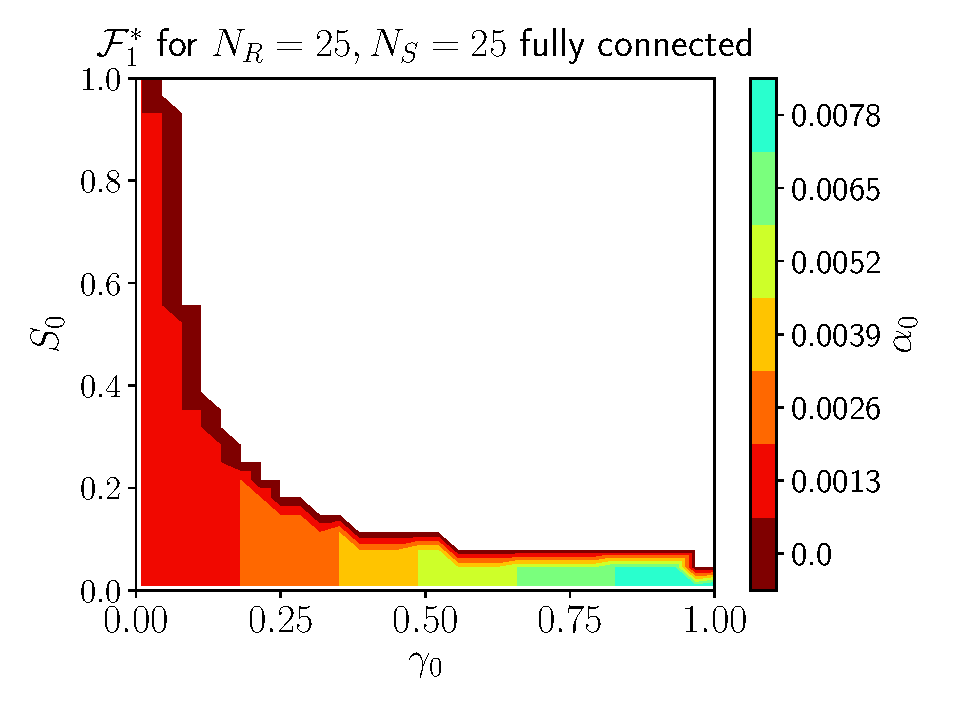
\includegraphics[width=0.6\linewidth]{common_feasibility_volume_NR25_NS25_varying_syntrophy_random_structure}}
% \subfloat[]{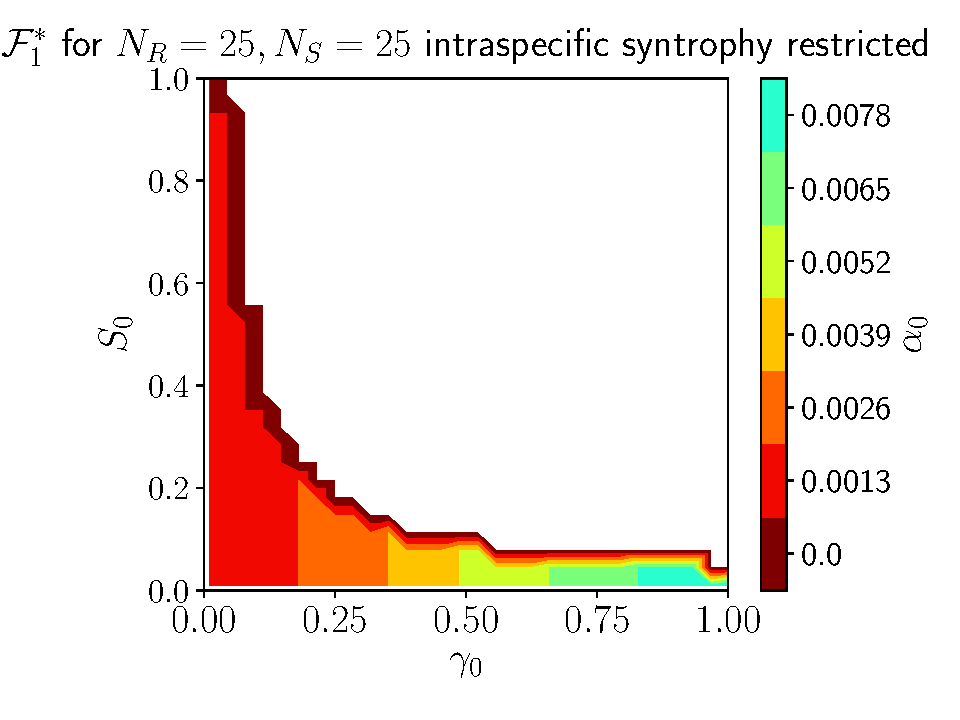
\includegraphics[width=0.6\linewidth]{common_feasibility_volume_NR25_NS25_varying_syntrophy_no_release_when_eat}}
%
% \centering
% \subfloat[]{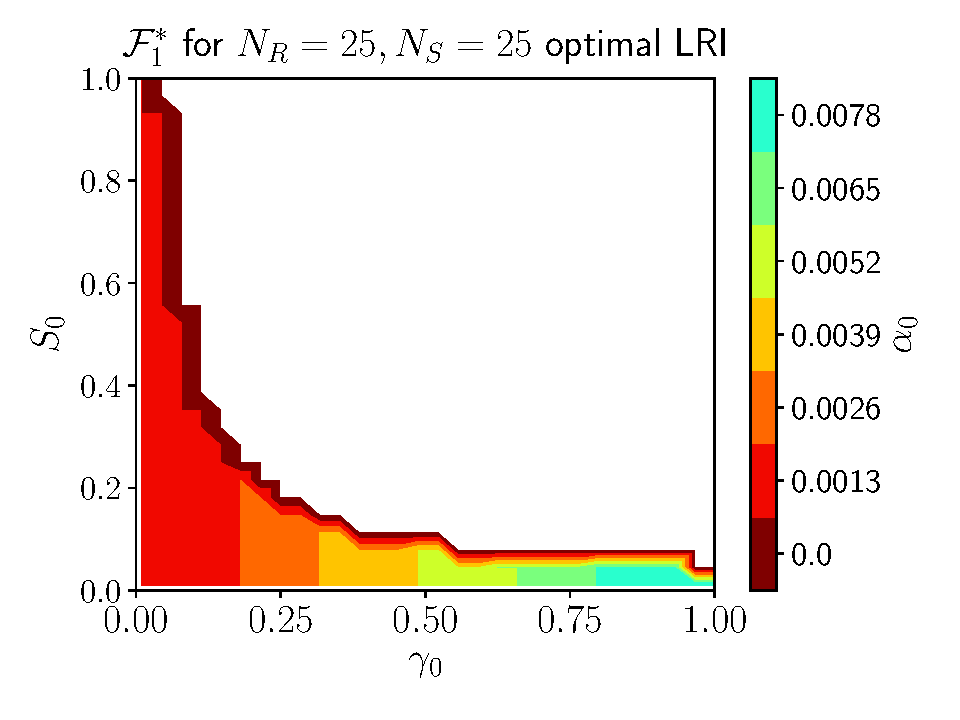
\includegraphics[width=0.6\linewidth]{common_feasibility_volume_NR25_NS25_varying_syntrophy_optimal_matrix}}
\hspace{-0.2\linewidth}
\includegraphics[width=1.4\linewidth]{{common_feasibility_region_NR25_NS25}.pdf}

\caption[caption for LOF]{Surface plot of the fully feasible volume $\mathcal{F}^{S_{25}}_1(\alpha_0)$. The color bar on the side indicates the value of $\alpha_0$ to which the surface corresponds. The white part of the plot corresponds to points that \important{never} are fully feasible. Note that even though it is not very clear on the figure $\mathcal{F}_1^{S_{25}}(\alpha_0^+) \subset \mathcal{F}_1^{S_{25}}(\alpha_0^-) \ \forall \alpha_0^+ > \alpha_0^-$, \ie the common fully feasible region of higher syntrophy is included in the one of lower syntrophy. The different subplots correspond to the different structures of the syntrophy matrix.} \label{fig: results feasibility cfv variation with syntrophy}
\end{figure}
\begin{figure}
\centering
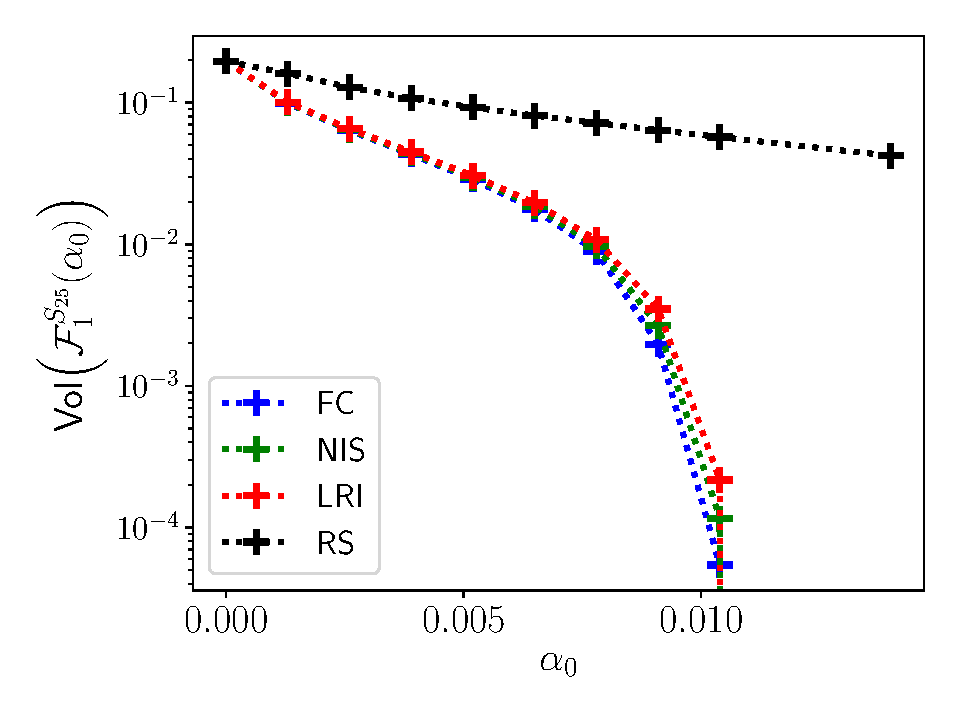
\includegraphics[width=0.65\linewidth]{common_feasibility_volume_NR25_NS25}
\caption{Volume of the common feasibility region $\mathcal{F}^{S_{25}}_1(\alpha_0)$ as a function of syntrophic interaction strength $\alpha_0$ (plotted on logarithmic scale). While the FC, NIS and LRI cases offer similar results, the RS scenario outperforms all of them. An exponential fit (Eq.\ref{eq: feasibility results fit feasible volume}) allows to measure a global $d_F$ for each of the four scenarios. The global decay feasibility rate of the RS scenario is 2.5 times smaller than the others.}\label{fig: feasibility results volume of cfr depending on syntrophy}
\end{figure}

\begin{figure}
\vspace{-120pt}
\hspace{-0.05\linewidth}
\subfloat[\label{fig: feasibility results feasibility region eta 0.6 kappa 0.3}]{\includegraphics[width=1.1\linewidth]{{feasibility_region_wt_NR50_NS25_Nest0.6_Conn0.3344}.pdf}}

\vspace{-28pt}
\hspace{-0.05\linewidth}
\subfloat[]{\includegraphics[width=1.1\linewidth]{{feasibility_region_wt_NR50_NS25_Nest0.35_Conn0.2296}.pdf}}

\vspace{-28pt}
\hspace{-0.05\linewidth}
\subfloat[\label{fig: feasibility results feasibility region eta 0.15 kappa 0.12}]{\includegraphics[width=1.1\linewidth]{{feasibility_region_wt_NR50_NS25_Nest0.15_Conn0.12}.pdf}}
\vspace{-12pt}
\caption{Surface colour plot of the fully feasible region $\mathcal{F}_1^{G,A}\left(\alpha_0\right)$ as a function of the syntrophy $\alpha_0$ for the case $N_R=50$, with different structures of $A$: fully connected (left column), no intraspecific syntrophy (middle) and LRI matrix (right). The rows correspond to different choices of the consumption matrix $G$: (a) $\eta_G=0.6$ and $\kappa_G=0.33$, (b) $\eta_G=0.35$ and $\kappa_G=0.23$, (c) $\eta_G=0.15$ and $\kappa_G=0.12$. These are matrices with similar properties than  Fig.\ref{fig: feasibility results fully feasible volume different consumption matrices}, except that the number of resources is here doubled. This affects $\mathcal{F}_1^{G,A}\left(\alpha_0\right)$ quite drastically.}\label{fig: feasibility results typical feasible volumes NR=50 NS=25}
\vspace{-60pt}
\end{figure}
\begin{figure}[h!]
\captionsetup[subfigure]{captionskip = -185pt, margin = 195pt}

\hspace{-0.1\linewidth}
\subfloat[]{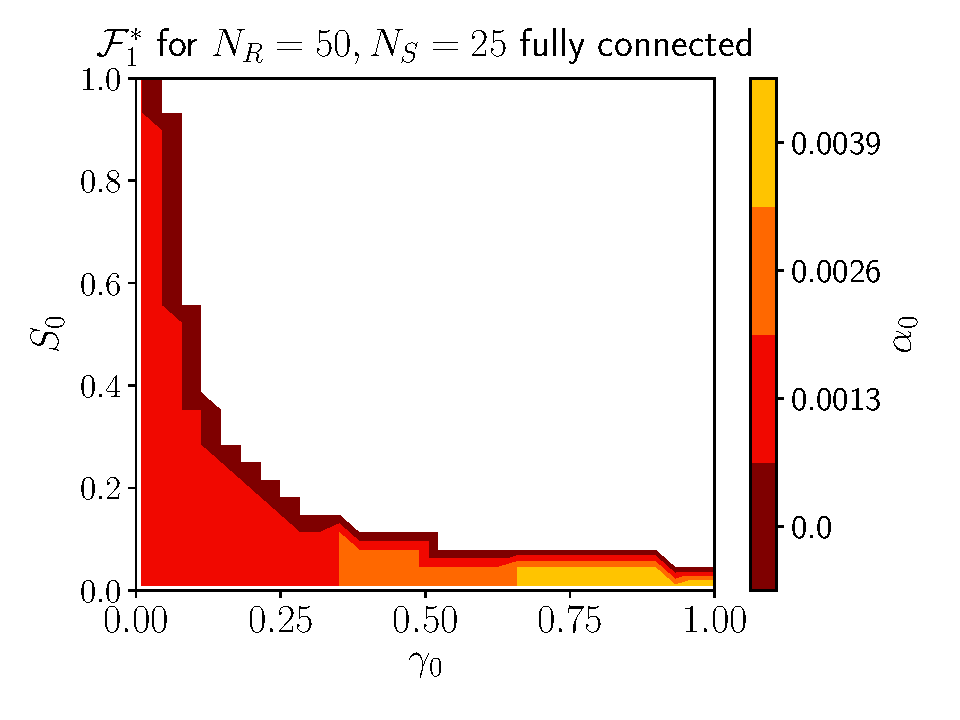
\includegraphics[width=0.6\linewidth]{common_feasibility_volume_NR50_NS25_varying_syntrophy_random_structure}}
\subfloat[]{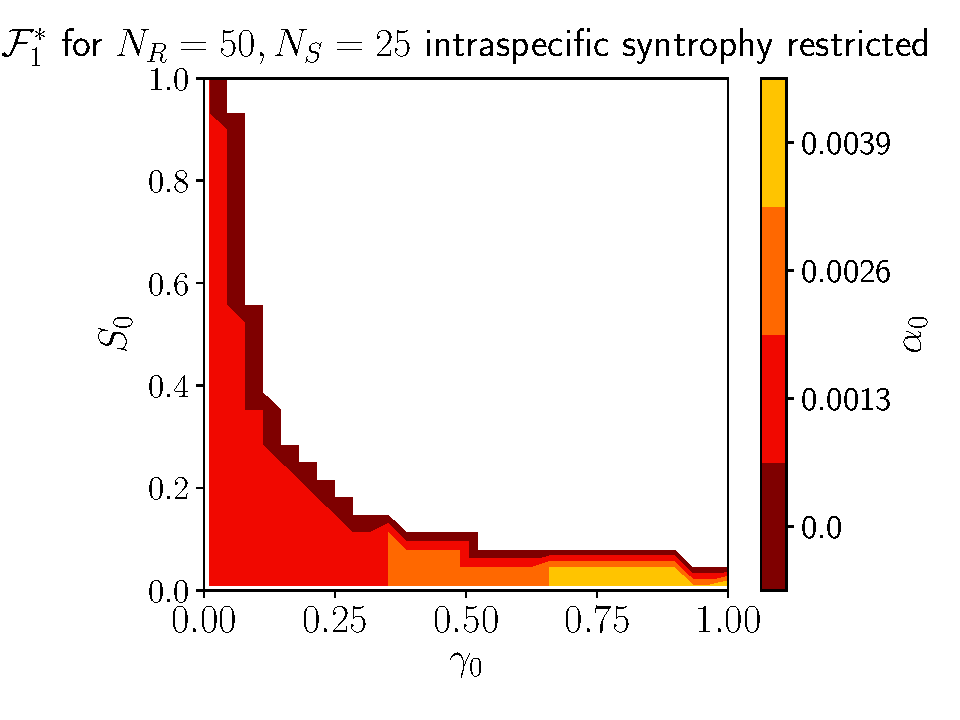
\includegraphics[width=0.6\linewidth]{common_feasibility_volume_NR50_NS25_varying_syntrophy_no_release_when_eat}}

\centering
\subfloat[]{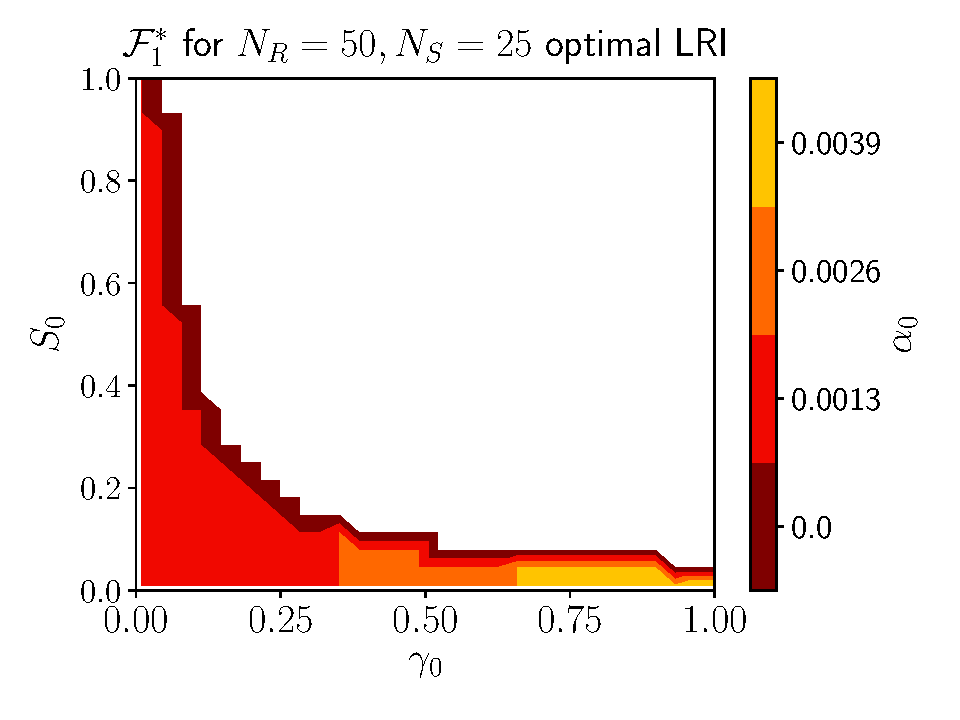
\includegraphics[width=0.6\linewidth]{common_feasibility_volume_NR50_NS25_varying_syntrophy_optimal_matrix}}
\caption{Common feasibility region $\mathcal{F}_1^{S_M}\left(\alpha_0\right)$ for $N_R=50$ and $N_S=25$, to compare with \ref{fig: results feasibility cfv variation with syntrophy}. We considered different structures of the syntrophy matrix: (a) fully connected, (b) intraspecific syntrophy restricted and (c) LRI matrix. As the number of resources increases, the feasibility volume for a given $\alpha_0$ decreases.}\label{fig: feasibility results common feasibility region NR=50 NS=25}
\end{figure}

\begin{figure}
\vspace{-84pt}
\captionsetup[subfigure]{captionskip=-202pt, margin=45pt}
\hspace{-0.1\linewidth}
\subfloat[]{\includegraphics[width=0.6\linewidth]{{feasibility_decay_rate_50_vs_25_fixed_connectance_fully_connected}.pdf}}
\subfloat[]{\includegraphics[width=0.6\linewidth]{{feasibility_decay_rate_50_vs_25_fixed_nestedness_fully_connected}.pdf}}

\hspace{-0.1\linewidth}
\subfloat[]{\includegraphics[width=0.6\linewidth]{{feasibility_decay_rate_50_vs_25_fixed_connectance_no_release_when_eat}.pdf}}
\subfloat[]{\includegraphics[width=0.6\linewidth]{{feasibility_decay_rate_50_vs_25_fixed_nestedness_no_release_when_eat}.pdf}}

\hspace{-0.1\linewidth}
\subfloat[]{\includegraphics[width=0.6\linewidth]{{feasibility_decay_rate_50_vs_25_fixed_connectance_optimal_matrix}.pdf}}
\subfloat[]{\includegraphics[width=0.6\linewidth]{{feasibility_decay_rate_50_vs_25_fixed_nestedness_optimal_matrix}.pdf}}

\vspace{-12pt}
\hspace{-0.1\linewidth}
% \subfloat[]{\includegraphics[width=0.6\linewidth]{{feasibility_decay_rate_50_vs_25_fixed_connectancerandom_structure}.pdf}}
% \subfloat[]{\includegraphics[width=0.6\linewidth]{{feasibility_decay_rate_50_vs_25_fixed_nestednessrandom_structure}.pdf}}

\caption{Ratio of the feasibility decay rates at $N_R=25$ and at $N_R=50$ as a function of the consumption matrix properties. A $y$-axis larger than $1$ means $d_F(N_R=25)$ is larger than $d_F(N_R=50)$, which means the system endures the addition of syntrophic interaction better at $N_R=50$. We considered the four usual $A$ scenarios (a)-(b) FC, (c)-(d) NIS, (e)-(f) LRI and (g)-(h) RS. Increasing the number of resources in the system does not allow microbial communities to be ``more feasible'' as syntrophy increases: on average $d_F$ is unchanged by doubling the number of resources. A detailed on how the consumption matrix properties, at least connectance and ecological overlap, or the $A$-scenario precisely modify the improvement is difficult to draw from this data.\textbf{TO DO: put also the one for random structure}}
\label{fig: feasibility results feasibility decay rate NR=50 NS=25}
\end{figure}
\end{document}
